
\documentclass[useAMS, usenatbib, referee]{biom}\usepackage[]{graphicx}\usepackage[]{color}
%% maxwidth is the original width if it is less than linewidth
%% otherwise use linewidth (to make sure the graphics do not exceed the margin)
\makeatletter
\def\maxwidth{ %
  \ifdim\Gin@nat@width>\linewidth
    \linewidth
  \else
    \Gin@nat@width
  \fi
}
\makeatother

\definecolor{fgcolor}{rgb}{0.345, 0.345, 0.345}
\newcommand{\hlnum}[1]{\textcolor[rgb]{0.686,0.059,0.569}{#1}}%
\newcommand{\hlstr}[1]{\textcolor[rgb]{0.192,0.494,0.8}{#1}}%
\newcommand{\hlcom}[1]{\textcolor[rgb]{0.678,0.584,0.686}{\textit{#1}}}%
\newcommand{\hlopt}[1]{\textcolor[rgb]{0,0,0}{#1}}%
\newcommand{\hlstd}[1]{\textcolor[rgb]{0.345,0.345,0.345}{#1}}%
\newcommand{\hlkwa}[1]{\textcolor[rgb]{0.161,0.373,0.58}{\textbf{#1}}}%
\newcommand{\hlkwb}[1]{\textcolor[rgb]{0.69,0.353,0.396}{#1}}%
\newcommand{\hlkwc}[1]{\textcolor[rgb]{0.333,0.667,0.333}{#1}}%
\newcommand{\hlkwd}[1]{\textcolor[rgb]{0.737,0.353,0.396}{\textbf{#1}}}%
\let\hlipl\hlkwb

\usepackage{framed}
\makeatletter
\newenvironment{kframe}{%
 \def\at@end@of@kframe{}%
 \ifinner\ifhmode%
  \def\at@end@of@kframe{\end{minipage}}%
  \begin{minipage}{\columnwidth}%
 \fi\fi%
 \def\FrameCommand##1{\hskip\@totalleftmargin \hskip-\fboxsep
 \colorbox{shadecolor}{##1}\hskip-\fboxsep
     % There is no \\@totalrightmargin, so:
     \hskip-\linewidth \hskip-\@totalleftmargin \hskip\columnwidth}%
 \MakeFramed {\advance\hsize-\width
   \@totalleftmargin\z@ \linewidth\hsize
   \@setminipage}}%
 {\par\unskip\endMakeFramed%
 \at@end@of@kframe}
\makeatother

\definecolor{shadecolor}{rgb}{.97, .97, .97}
\definecolor{messagecolor}{rgb}{0, 0, 0}
\definecolor{warningcolor}{rgb}{1, 0, 1}
\definecolor{errorcolor}{rgb}{1, 0, 0}
\newenvironment{knitrout}{}{} % an empty environment to be redefined in TeX

\usepackage{alltt}
\usepackage{appendix, subfigure}
\usepackage{framed}
%\usepackage{authblk}
\usepackage{bm,amsmath}
\usepackage{amsfonts}
%\usepackage{hyperref}
\usepackage{blkarray}
\usepackage[colorinlistoftodos,linecolor=gray,backgroundcolor=white]{todonotes}

% my command definitions
%\newtheorem{exercise}{Exercise}[chapter]
%\newtheorem{example}{Example}[chapter]
\newcommand{\ol}[1]{\overline{#1}}
\newcommand{\D}{\displaystyle}
\newcommand{\T}{\textstyle}
\newcommand{\s}{\scriptstyle}
\newcommand{\mc}[1]{\mathcal{#1}}
\newcommand{\bex}{\begin{exercise}}
\newcommand{\eex}{\end{exercise}}
\newcommand{\beg}{\begin{example}}
\newcommand{\eeg}{\end{example}}
\newcommand{\schist}[1]{\mbox{\tiny{#1}}}
\newcommand{\chist}[1]{\mbox{\scriptsize{#1}}}
\newcommand{\agemo}[1]{\mbox{$\underline{\omega}_{\/\downarrow #1}$}}
\newcommand{\ul}[1]{\mbox{$\underline{#1}$}}
\newcommand{\wh}[1]{\mbox{$\widehat{#1}$}}
\newcommand{\bv}{\begin{verbatim}}
\newcommand{\ev}{\end{verbatim}}
\newcommand{\bi}{\begin{itemize}}
\newcommand{\ei}{\end{itemize}}
\newcommand{\bfig}{\begin{figure}}
\newcommand{\efig}{\end{figure}}
\newcommand{\pref}[1]{\protect\ref{#1}}
\newcommand{\plab}[1]{\protect\label{#1}}
\newcommand{\be}{\begin{eqnarray}}
\newcommand{\bes}{\begin{eqnarray*}}
\newcommand{\ee}{\end{eqnarray}}
\newcommand{\ees}{\end{eqnarray*}}
\newcommand{\bo}[1]{\bf #1}
\newcommand{\bmt}[1]{\mbox{\boldmath $#1$}}
\newcommand{\tm}[1]{\mbox{\tiny{$#1$}}}
\newcommand{\vc}[2]{\mbox{$ \left[ \begin{array}{c} #1\\ \vdots \\ #2 
 \end{array} \right] $}}
\newcommand{\mt}[4]{\mbox{$ \left[ \begin{array}{c,c,c} #1 & \cdots & #2\\ 
 \vdots & \ddots & \vdots\\ #3 & \cdots & #4 \end{array} \right] $}}

\setcounter{footnote}{2}



\IfFileExists{upquote.sty}{\usepackage{upquote}}{}
\begin{document}

\title{A model for digital aerial surveys of marine mammals without individual identification}

\author{D. L. Borchers\(^{1, *}\)\email{dlb@st-andrews.ac.uk},
P. Nightingale\(^1\),
B.C. Stevenson\(^{2}\), and
R.M. Fewster\(^{2}\) \\
\(^1\)University of St Andrews, Centre for Research into Ecological and Environmental Modelling, \\ St Andrews, Fife, UK \\
\(^2\)Department of Statistics, University of Auckland, Private Bag 92019, \\ Auckland, New Zealand
}
%\author[1]{D.L. Borchers\thanks{dlb@st-andrews.ac.uk}}
%\author[2]{P. Nightingale}
%\author[3]{B.C. Stevenson}
%\author[3]{R.M. Fewster}
%\affil[1]{Centre for Research into Ecological and Envoronmental Modelling
%University of St Andrews, The Observatory, Buchanan Gardens, Fife, St Andrews, KY16 9LZ, Scotland}
%\affil[2]{School of Computer Science, Jack Cole Building
%North Haugh, St Andrews, Fife, KY16 9SX, Scotland}
%\affil[3]{Department of Statistics, University of Auckland,
%Private Bag 92019, Auckland, New Zealand}




\date{{\it Received ??} 2018. {\it Revised } 20??}
%{\it Accepted March} 2005.}

\pagerange{\pageref{firstpage}--\pageref{lastpage}} \pubyear{2018}

\volume{00}
\artmonth{??}
\doi{10.1111/j.1541-0420.2005.00454.x}

%  This label and the label ``lastpage'' are used by the \pagerange
%  command above to give the page range for the article

\label{firstpage}

%  pub the summary here

\begin{abstract}
Yadda, yadda, yadda, ...
\end{abstract}

\begin{keywords}
Keywords: Double-observer, Mark-recapture, line transect, availability bias, movement model, Poisson process
\end{keywords}


\maketitle

\section{Introduction}\label{sec:intro}

Aerial surveys of marine mammals are generally much cheaper than shipboard surveys. We anticipate that aerial surveys with human observers will increasingly be replaced by unmanned aerial vehicle (UAV) surveys with digital video or still cameras as observers. Such surveys present some new statistical challenges. In this paper we address these challenges and develop a method of estimating animal density from a UAVs carrying cameras.

Animals are within detectable range of an observer on an aircraft for only a short time, because aircraft move fast. Some animals are missed from an aircraft because they are underwater and unobservable while within detection range. This is known as the ``$g(0)<1$'' problem in the line transect literature \textbf{add citation} and the bias that results from ignoring this problem is often called ``availability bias'' \textbf{add citation}. UAVs with digital cameras will tend to miss more animals than for aircraft with humans because the cameras typically have much smaller fields of view: perhaps 100m either side of the survey transect line, compared with 1000m or more for human observers.

Mark-recapture distance sampling (MRDS) methods \textbf{add citation} are commonly used to deal with the ``$g(0)<1$''  problem. These methods are a variety of capture-recapture method, in which two independently searching observers constitute two ``capture occasions'' and animals detected by both constitute ``recaptures''. 

MRDS methods on aerial surveys suffer from the fact that two observers on the same aircraft search the same patch of sea at the same time so that animals tend to be available or unavailable to both observers at the same time. This induces positive correlation in the detection events between the observers, and negative bias in density estimates \textbf{add citation}. (For those familiar with capture-recapture models, you can think of the availability state of an animal as an individual-level latent variable: when there is unmodelled individual heterogeneity on capture-recapture surveys, density estimates are biased.) 

There are two ways in which this problem has been dealt with. The first is to model the latent process, i.e., the availability process. For example, \textbf{(citations)} modelled latent availability using a hidden Markov model, while \textbf{(citations)} modelled it using a Markov modulated Poisson processes. The second way is to separate the times that the two observers search the same region, either by having one observer search far ahead of the aircraft and the other close to it, or by using two aircraft in tandem, or having a single aircraft circle back over its path a second time \citep[see][(need to add others too?)]{Hiby+Lovell:98}.

However, separating the observers in this way has a cost: it introduces uncertainty into capture histories.

MRDS methods require that every detected individual be identified as having been detected by observer 1 only (capture history (1,0)), observer 2 only (capture history (0,1)), or both observers (capture history (1,1)). Because marine mammals are generally not individually identifiable from a fast-moving aerial survey platform, it is often not possible to obtain these capture histories without error. 

The greater the time separation between observers, the more severe is the problem of errors in capture histories, but the less severe the problem of dependence in detections.

Separating UAV ``observers'' (cameras) by using UAVs in tandem or circling back on themselves is much less feasible than doing the same with human observers on aircraft. This is because field conditions are typically such that it is not possible for the aircraft doing the second pass to follow exactly the path of the aircraft doing the first pass. When observer field of view is around 2,000m wide (as is not unusual with human observers), having a second pass that deviates by 200m from the path of the first pass still leaves considerable overlap between the regions surveyed by each observer. It would leave no overlap at all for UAVs with a field of view 200m wide. 

We seek a method that allows a single UAV to carry two cameras. This limits the extent to which the two observers can be separated in time and requires that we deal with dependence between detections resulting from cameras passing in quick succession. We develop a method that does not require capture histories to be assigned to any individuals and deals with dependence by modelling the availability process. 

Our method is similar to that of \cite{Stevenson+al:18} in that it has the same data requirements and does not require capture histories. It differs in that we do inference by maximum likelihood rather than using an approximation to the Palm likelihood. Unlike the method of \cite{Stevenson+al:18}, our method becomes computationally infeasible when there are very many plausible pairings of detections by different observers. It is also similar to that of \cite{Hiby+Lovell:98}, which suffers from the same computational restriction. We investigate its utility for aerial UAV surveys and compare it to the method of \cite{Stevenson+al:18}. 

\section{The model\label{sec:genmod}}


\subsection{The movement model}

Two observers move along a transect line, one behind the other moving at $v$ m/s, separated by a distance $vl$. Animals may move between the time that the first and second observers pass them. 

We model animal movement in time $t$, as a bivariate normal distribution with mean $(0,0)$ and variance $\Sigma(t)=\sigma^2t\bm{I}$, where $\bm{I}$ is a $2\times 2$ identity matrix. This model is consistent with movement that is Brownian motion. It is straightforward to introduce directionality by replacing the zero off-diagonal elements of $\bm{I}$ with a correlation parameter $\rho$, although we do not do that here.

\subsubsection{Forward movement}

In Appendix~\ref{appx:firstpassage} we show that when the two observers are moving at a speed $v$ separated by time lag $l$, the pdf of the time between the first and second observers encounter an animal ($T$), is 
\be
%f_Y(y)&=&\frac{f_B(y;\sigma^2t)}{\int_{-\infty}^{\infty}f_B\left(\frac{uy}{t};\sigma^2u\right)du}
f_{T}(t)&=&\frac{vl\exp\left\{-\frac{v^2(l-t)^2}{2\sigma^2t}\right\}}{\sqrt{2\pi\sigma^2t^3}}.
\ee

The animal will have moved a forward distance $v(t-l)$ in this time, with negative distance being movement in the opposite direction to that of the observers, and positive distance being in the same direction.

%It follows that the distance $y=vt$ that the animal has moved in the forward direction when the second observer passes it is 
%\be
%f_{Y|k}(y|k)&=&\frac{vl\exp\left\{-\frac{(vl-y)^2}{2\sigma^2y/v}\right\}}{\sqrt{2\pi\sigma^2y^3/v}}.
%\ee


\subsection{Availability models}

There are two reasons that animals that are within the survey strip at some point between the passing of the first and second observers may not be available for detection. The first is that they are invisible to the observers because they are diving. The second is that they are invisible because they are not within the strip at the time they are passed. We construct models for each of these processes below. 

\subsubsection{The up/down availability model}

We assume animals unavailability due to diving is governed by a two-state continuous time Markov process with transition intensity matrix parameters such that the time in state 1 (the near-surface state) is an exponential random variable with expected value $\kappa$, and the time in state 2 (the diving state) is an exponential random variable with expected value $\tau-\kappa$, where $\tau$ is the expected dive cycle duration:

The Markov transition rate matrix $\bm{Q}$ is
\be
\bm{Q}&=&
\left(
\begin{array}{cc}
-\frac{1}{\kappa} & \frac{1}{\kappa} \\
\frac{1}{\tau-\kappa} & -\frac{1}{\tau-\kappa}
\end{array}
\right)
\label{eq:Q}
\ee
\noindent
from which it follows that the stationary distribution of the Markov chain is 
\begin{eqnarray}
\underline{\pi}
&=&
%\left(\frac{q_{22}}{q_{22}+q_{11}},\frac{q_{11}}{q_{11}+q_{22}}\right)
%\;=\;
\left(\frac{\kappa}{\tau},\frac{\tau-\kappa}{\tau}\right).
\end{eqnarray}
\noindent

\noindent
The transition probability matrix for transitions between states at time separation $t$ is $\bm{U}(t)=\exp(\bm{Q}t)$.


\subsubsection{The in/out availability model}


Suppose both observers search a distance $w$ either side of the transect line. We consider a strip of half-with $b>w$, such that there is zero, or neglibly small probability that an animal outside this strip when the first observer passes, moves to within $w$ of the transect in the time between the two observers coming abeam of the animal. For each animal that is within $b$ of the transect when observer 1 passes it, we define the binary random variable $Z(t)$ to be 1 if the animal is within $w$ of the transect at time $t$ after the first observer passes it, and is zero otherwise. For notational convenience, we define $\bar{Z}_j=1-Z_j$. Under the above movement model for $X(t)$, the probability $\mathbb{P}(Z(t)=0|Z(0)=1)$, that an animal moves from inside the searched strip to outside it in an interval $t$, and the probability $\mathbb{P}(Z(t)=1|Z(0)=0)$, that it moves from outside the searched strip to inside it, are 

\be
p_{IO}(t)=\mathbb{P}(Z(t)=0|Z(0)=1)&=&\frac{1}{w}\int_0^w\Phi(x-w;\sigma^2t)+\Phi(-x-w;\sigma^2t)dx
\label{eq:p_{IO}}\\
p_{OI}(t)=\mathbb{P}(Z(t)=1|Z(0)=0)&=&\frac{1}{b-w}\int_w^{b}\Phi(x-w;\sigma^2t)-\Phi(-x-w;\sigma^2t)dx 
\label{eq:p_{OI}}
\ee
%\todo[inline]{Lifted from old notes without checking -- needs checking.}
\noindent
where $\Phi(\cdot;\sigma^2t)$ is the cumulative distribution function of a normal random variable with mean zero and variance $\sigma^2t$.

We model the movement in and out of the survey strip as a two-state Markov process with transition probabilities at time $t$ after being passed by the first observer that are given by Eqns~\eqref{eq:p_{IO}} and \eqref{eq:p_{OI}}:

\be
\bm{M}(t)&=&
\left(
\begin{array}{cc}
1-p_{IO}(t) & p_{IO}(t) \\
p_{OI}(t) & 1-p_{OI}(t)
\end{array}
\right)
\label{eq:M}
\ee

\subsubsection{The combined availability model}

The possibility of being in the survey strip or outside it and on the surface or below it, gives rise to four states that animals can occupy: (up and in), (up and out), (down and in) and (down and out), which we now number 1 to 4 in that order. Assuming that being up or down is independent of being in or out, transitions between these states at a time separation $t$ is governed by the transition probability matrix $\bm{\Gamma}(t)=\bm{U}(t)\otimes\bm{M}(t)$.

%To obtain the initial state distribution, we consider a ``buffer'' of width $b\sigma T$ either side of the searched strip (of width $W$). We choose $b$ such that there is zero, or close to zero, probability of an animal beyond this buffer moving into the survey strip in a time $T$, and we choose $T$ such that there is zero, or nearly zero, probability of the time between observers passing an animal being greater than $T$.

Assuming uniform animal distribution with respect to the transect line at the time that the first observer passes animals, the probability that an animal that is within $b$ of the line, is in the searched strip is $w/b$. Combined with the stationary distribution $\pi$, this gives the following initial state distribution:
\be
\bm{\delta}&=&\left(
\frac{\kappa}{\tau}\frac{w}{b},\;
\frac{\kappa}{\tau}\left[1-\frac{w}{b}\right],\;
\left[\frac{\tau-\kappa}{\tau}\right]\frac{w}{b},\;
\left[\frac{\tau-\kappa}{\tau}\right]\left[1-\frac{w}{b}\right]
\right).
\label{eq:delta}
\ee



\section{A Markov modulated Bernoulli process model}

We assume that the probability that an animal is in each state at the time the first observer passes over it is given by the stationary distribution $\bm{\delta}$, and hence that its state distribution after a waiting time $t$, when the second observer passes it, is $\bm{\delta}\bm{\Gamma}(t)$. 

Each observer records binary variable $X_{ij}(t)$, which is 1 when the animal $i$ is detected by observer $j$ at time $t$ and is zero otherwise. We model $X_{ij}(t)$ as a state-dependent Bernoulli random variable with parameter $p_j(c)=\mbox{Pr}(X_{ij}(t)=1|C_i(t)=c)$ where $C_i(t)$ is the state of animal $i$ at time $t$ and $c\in(1,2,3,4)$. 

It follows that $X_{ij}(t_{ij})$ ($j=1,2$) are observations from a Markov modulated Bernoulli process (MMBP) at times $t_{i1}$ and $t_{i2}$. It is convenient to define the time at which the first observer passes animal $i$ ($t_{i1}$) to be zero, so that the time at which the second observer passes is $t_{i2}$ ($t$ in the development of the previous section).

It is convenient for the hidden Markov model formulation to arrange detection probabilities in a detection probability matrix. For observer $j$, this matrix is
\be
\bm{P}\{x_{ij}(t)\}\;=\;
\begin{blockarray}{cccc}
\text{up,in} & \text{up,out} & \text{down,in} & \text{down,out} \\ 
\begin{block}{(cccc)}
\text{Bern}(x_{ij}(t);p_j(1)) & 0 & 0 & 0 \\
0 & 1-x_{ij}(t) & 0 & 0 \\
0 & 0 & \text{Bern}(x_{ij}(t);p_j(3)) & 0 \\
0 & 0 & 0 & 1-x_{ij}(t) \\
\end{block}
\end{blockarray} 
\ee
\noindent
where $\text{Bern}(x_{ij}(t);p_j(c)\equiv p_j(c)^{x_{ij}(t)}[1-p_j(c)]^{1-x_{ij}(t)})$. In the above matrix we allow a more general case than we deal with below, in which it is possible to detect an animal that is within the survey strip and not in the near-surface state. In what follows we assume that only animals in the near-surface state can be detected so that $p_j(3)=0$.

Conditional on $t_{i2}$, and remembering that $t_{i1}$ is defined to be 0, the probability of observing $\{x_{i1}(0),x_{i2}(t_{i2})\}$, is 
\be
p\{x_{i1}(0),x_{i2}(t_{i2})|t_{i2}\}&=&
\bm{\delta}\bm{P}\{x_{i1}(0)\}\bm{\Gamma}(t_{i2})\bm{P}\{x_{i2}(t_{i2})\}\bm{1}
\ee
\noindent
where $\bm{1}$ is a column vector of ones. The joint probability of the second observer passing animal $i$ at $t_{i2}$ and observing $\{x_{i1}(0),x_{i2}(t_{i2})\}$ is $p\{x_{i1}(0),x_{i2}(t_{i2}|t_{i2})\}f_{T}(t_{i2})$. 

For brevity, we now write $p\{x_{i1}(0)=0,x_{i2}(t_{i2})=1|t_{i2}\}$ as $p_{01}(t_{i2})$, we write $p\{x_{i1}(0)=1,x_{i2}(t_{i2})=0|t_{i2}\}$ as $p_{10}(t_{i2})$, and we write $p\{x_{i1}(0)=1,x_{i2}(t_{i2})=1\}$ as $p_{11}(t_{i2})$.

Writing the three observable capture histories as $\omega_1=(01), \omega_2=(10), \omega_3=(11)\}$, we can write the probability of observing each of these as
\be
\tilde{p}_{\omega_k}=E_{t}[p_{\omega_k}(t)]&=&\displaystyle\int p_{\omega_k}(t)f_{T}(t)dt.
\ee
\noindent
for $k=1,2,3$.

\section{The survey model}

We assume that the number and locations of animals along the transect at the time of the first or second observer passing are governed by a nonhomogeneous Poisson process (NHPP) with rate paramter $D(s)$ at location $s$. We define the observed location of detected animal $i$ to be its location at the time the first observer passes it, or if it is not detected by the first observer, then at the time that the second observer passes it. 

Let $\bm{s}_{\omega}=(\bm{s}_{\omega_1},\bm{s}_{\omega_2},\bm{s}_{\omega_3})$ be the observed locations along the transect of detections with capture history $\omega_1=(01), \omega_2=(10), \omega_3=(11)$. These arise from thinned NHPPs with thinning probabilities $ \tilde{p}_{\omega_k}$ ($k=1,2,3$), so that for a survey along transects of total length $L$, the pdf of locations $\bm{s}_{\omega}$ is
\be
f(\bm{s}_{\omega})&=&\left[\prod_{i=1}^{n_{\omega}}\tilde{p}_{\omega} D(s_{\omega i})\right]e^{-\int_0^L\tilde{p}_{\omega} D(s)ds}.
\label{eq:f(s_omega)}
\ee
\noindent
where $n_{\omega}$ is the number of individuals with capture history $\omega$.

In the case of $\omega=(11)$, we also observe the time $t_{(11)i}$ between the two observers passing the $i$th animal with capture history $(11)$, for $i=1,\ldots,n_{(11)}$. (We do not observer these for capture histories (01) and (10).) The pdf for the $i$th of these is the conditional pdf of time between passing, given that the capture history is $(11)$. This is
\be
f_{T|11}(t_{(11)i},\omega_i=11)&=&\frac{f_{T}(t_{(11)i})p_{11}(t_{(11)i})}{\tilde{p}_{11}}.
\ee
%\noindent
%where $p_{11}(k+\delta_{(11)_i}|X_{i1}(0)=1)$ and $\tilde{p}_{11}(k|X_{i1}(0)=1)$ are 
%\be
%p_{11}(k+\delta_{(11)i}|X_{i1}(0)=1)&=&
%(1,0)\exp\{\bm{Q}(k+\delta_{(11)i})\}\bm{P}\{X_{i2}(k+\delta_{(11)i})=1\}\underline{1} \nonumber \\
%\mbox{and}\;\;\;\tilde{p}_{11}(k|X_{i1}(0)=1)&=&\displaystyle\int p_{11}(k+\delta|X_{i1}(0)=1)f_\delta(\delta;k)d\delta \nonumber
%\ee

We assume that the $t_{(11)i}$s are independent ($i=1,\ldots,n_{(11)}$).% \footnote{Note to self: when $p_j(1)=p_j(2)=1$ then $f_{\delta_{11}}(\delta_{(11)i};k)=f_\delta(\delta_{(11)i};k)$ and so likelihood \texttt{negllik} is evaluated with \texttt{sp=TRUE} is identical to it evaluated with \texttt{sp=FALSE}.}

Given the capture histories $\bm{\omega}$, the likelihood is therefore as follows (with model parameters suppressed for simplicity of presentation):
\be
\mathcal{L}(\bm{s}|\bm{\omega})&=&\left\{\prod_\omega\left[\prod_{i=1}^{n_\omega}\tilde{p}_\omega D(s_{\omega i})\right]e^{-\int_0^L\tilde{p}_\omega D(s)ds}\right\}
\prod_{i=1}^{n_{(11)}}f_{T| 11}(t_{(11)i}| \omega_i=11) \nonumber \\
&=&e^{-\int_0^L\tilde{p}_\cdot D(s)ds}\left\{\prod_\omega \tilde{p}_\omega^{n_\omega}\prod_{i=1}^{n_\omega}D(s_{\omega i})\right\}
\prod_{i=1}^{n_{(11)}}f_{T|11}(t_{(11)i}|\omega_i=11) 
\label{eq:f(s)}
\ee
\noindent
where $\bm{\omega}$ is the set of capture histories of each detection, $\prod_\omega$ means the product over $\omega\in\{(10),(01),(11)\}$, $\tilde{p}_\cdot=\sum_\omega \tilde{p}_\omega$, and $\bm{s}=(\bm{s}_{(10)},\bm{s}_{(01)},\bm{s}_{(11)})$.

\subsection{Homogeneous Poisson case}

In the homogeneous Poisson case, when $D(s)=D$
\be
\mathcal{L}(\bm{s}|\bm{\omega})
&=&
e^{-\tilde{p}_\cdot DL}D^n\left(\prod_{\omega\in \{10,01,11\}} \tilde{p}_\omega^{n_\omega}\right)
\prod_{i=1}^{n_{(11)}}f_{T|11}(t_{(11)i}|\omega_i=11) \nonumber \\
&=&
e^{-\tilde{p}_\cdot DL}D^n\left(\prod_{\omega\in \{10,01\}} \tilde{p}_\omega^{n_\omega}\right)
\prod_{i=1}^{n_{(11)}}f_{T}(t_{(11)i})p_{11}(t_{(11)i})
\label{eq:f(s).D}
\ee
\noindent
where $n=\sum_\omega n_\omega$.
%In order to constrain $D$ to be non-negative, we parameterise it as $D=e^{\theta_1}$.

\subsection{Model parameters}

The model has four kinds of parameters:

\textbf{Density parameters}: In the case of the homogenous Poisson process there is one parameter, $\theta$ such that $D=e^{\theta}$. When density varies with some covariates, $\theta$ is replaced by a linear predictor involving a parameter vector.

\textbf{Dive cycle parameters}: The two-state dive cycle model described above involves the mean time in the near-surface state, $\mu_1$, and the mean dive cycle length, $\tau$, which are linked to parameters $\gamma_1$ and $\gamma_\tau$ via a log link: $\mu_1=e^{\gamma_1}$ and $\tau=e^{\gamma_\tau}$.

\textbf{Movement parameters}: The movement model has one parameter, $\sigma$, which we model using a log link: $\sigma=e^\phi$.

\textbf{Detection parameters}: Assuming that animals are only detectable when in state $c=1$ (up,in), we have two Bernoulli parameters to model: $p_1(1)$ and  $p_2(1)$. These can be modelled using logit link functions and if the observers are identical digital detectors it may be reasonable to assume these two probabilities are identical, i.e. $p_1(1)=p_2(1)=p=e^\beta/(1+e^\beta)$.

As is the case with density parameters, the other three kinds of parameters can be modelled as functions of suitable covariates by replacing the relevant scalar parameter on the link scale with a suitable linear predictor involving the covariates.

We focus on the constant density model in the rest of this paper. With no covariates, it has five parameters, which we write as $\bm{\theta}^*=(\theta,\gamma_1,\gamma_\tau, \phi, \beta)$. \cite{Stevenson+al:18} show that not all of these parameters are identifiable. They assume that $p=e^\beta/(1+e^\beta)=1$, and we do the same. This is reasonable for digital aerial surveys conducted in low sea states if we define the near-surface state to be ``breaking the surface'' (a state that is easily observed). The field of view of digital cameara is such that objects towards the periphery of the image are as easily detected as objects in the centre of the image so that a detection function of the sort used on line transect surveys, i.e., one that drops off with distance from the line, is not needed. 

\cite{Stevenson+al:18} show that even in this case, only two of $(\theta,\gamma_1,\gamma_\tau)$ are identifiable. Like  \cite{Stevenson+al:18} and \cite{Hiby+Lovell:98}, we specify the mean dive cycle duration, $\tau=e^{\gamma_\tau}$ on the basis of estimates external to the survey. In what follows, we assume certain detection of animals that are on the surface when in view, use external estimates to set $\tau$, and estimate the density, $D$, the mean time in surface state, $\mu_1$, and the Brownian movement parameter, $\sigma$, That is, we estimate $\bm{\theta}=(\theta,\gamma_1, \phi)$). We do this using the locations along the transect line of detections by the first observer and the locations along the transect line of detections by the second observer (and known observe speed) without assigning capture histories to any individual.

\section{Unknown capture histories}

If we knew which animals had capture histories (10), (01) and (11) (i.e., we were given $\bm{\omega}$), we could estimate the model parameters by maximising the likelihood Equation~(\ref{eq:f(s).D}) with respect to $\bm{\theta}$.

However, we don't know which animals have which capture histories. Following \cite{Hiby+Lovell:98} we marginalise over the (unknown) capture histories by summing the likelihoods for all possible capture history combinations. We refer to each combination as a ``pairing'' since once the pairs of detections with capture history (11) have been determined, this determines the capture histories of all detections -- because we know for each of the other detections which one of the two observers made the detection.

If we call the $m$th set of pairings $\bm{\omega}^{(m)}$, we can consider $\mathcal{L}(\bm{\theta};\bm{s}|\bm{\omega}^{(m)})$ to be the conditional likelihood, given $\bm{\omega}^{(m)}$, and we obtain the unconditional likelihood for the parameters $\bm{\theta}$ as
\be
\mathcal{L}(\bm{\theta};\bm{s})&=&\sum_{m=1}^M\mathcal{L}(\bm{\theta};\bm{s}|\bm{\omega}^{(m)})
\ee
\noindent
where $M$ is the number of possible pairings.

While this likelihood is easy to write down, it is challenging to evaluate because we need to enumerate all possible $\bm{\omega}^{(m)}$s, and for any but very small sample sizes, the number $M$ of possible pairings is very large ($M>>10^9$ for even moderate sample sizes).

We use constraint programming methods (see Section~\ref{sec:constrprog}) to efficiently find all possible pairings, and subdivision of $\bm{s}$ into subsets between which pairings of detections by different observers is impossible, to reduce the number of possible pairings.

\subsection{Subdivision of $\bm{s}$}

We subdivide $\bm{s}$ by ``cutting'' the transect line immediately after detections by observer $j$ for which the distance to the next detection by observer $(3-j)$ is greater than a maximum possible distance that an animal could have moved between the two observers passing over it ($d_{max}$). This distance $d_{max}$ must be decided by the user in the light of knowledge of the target species movement speed and behaviour. Users can investigate what $d_{max}$ is reasonable by doing inference at a range of plausible values to find where estimates become insensitive to $d_{max}$. The cost of setting $d_{max}$ too large is in computational speed; the cost of setting $d_{max}$ too small is positive bias in estimation of $D$ since too small a $d_{max}$ will result in some animals with true capture history (11) being assigned capture history (01) or (10).

Having divided the transect line into $C$ segments, we enumerate the possible parings $\bm{\omega}^{(m_c)}$ for segments $c=1,\ldots,C$ (with $M_c$ possible pairings in segment $c$) and calculate the likelihood as 
\be
\mathcal{L}(\bm{\theta};\bm{s})&=&\prod_{c=1}^C\sum_{m_c=1}^{M_c}\mathcal{L}(\bm{\theta};\bm{s}|\bm{\omega}^{(m_c)})
\ee

When $d_{max}$ is substantially smaller than most of the distances between detections by different observers, segmentation can lead to a massive reduction in computation time, making an otherwise computationally infeasible likelihood evaluation quite feasible. If $d_{max}$ is not substantially smaller than a large fraction of the distances between detections by different observers, and sample sizes are not very small, computation of the likelihood may be so time consuming as to render the method practically useless.

\subsection{Enumerating all $\bm{\omega}^{(m)}$s}
\label{sec:constrprog}

To enumerate the possible pairings within one segment efficiently we define a simple \textit{constraint satisfaction problem} (CSP)~\cite[Chapter 6]{russell-norvig-aima3}. A CSP is a triple \(\mathcal{X}=\langle \mathcal{V}, \mathcal{D}, \mathcal{C} \rangle\).  The CSP \(\mathcal{X}\) has a set of decision variables \(\mathcal{V}\), each of which has a set of possible values that it may take, called its \textit{domain}, where \(\mathcal{D}(x)\) is the domain of \(x \in \mathcal{V}\). In addition a CSP has a set of constraints \(\mathcal{C}\) that restrict the combinations of values that may be taken by the variables. A constraint \(c\in \mathcal{C}\) is a relation defined on a set of variables \(\mathrm{scope}(c)\subseteq \mathcal{V}\). A \textit{solution} is an assignment of values to variables such that each variable is assigned a value from its domain, and all constraints are satisfied. 

We define a CSP for a segment as follows. 
Two detections by different observers may be paired iff the distance between them is less than or equal to \(d_{max}\). For each set \(\{i,j\}\) of two observations that may be paired we define one decision variable \(b_{i,j}\) with domain \(\{0,1\}\). Variable \(b_{i,j}\) is equal to 1 in a solution iff the two observations are paired. 

Suppose we have two sets, \(s_1=\{i,j\}\) and \(s_2=\{k,l\}\), where \(s_1 \cap s_2 \ne \emptyset\), \(i\) may be paired with \(j\), and \(k\) may be paired with \(l\). The two sets cannot both be paired simultaneously because they share an observation. In all such cases we add the constraint \(b_{i,j}=0 \vee b_{k,l}=0\) to prevent both sets being paired simultaneously. 

We use a backtracking search procedure with forward checking~\cite[Chapter 6]{russell-norvig-aima3} to enumerate all solutions to the CSP. The set of solutions to the CSP correspond one-to-one to the set of valid pairings within the segment. When a solution is found, the part of the likelihood pertaining to that pairing is calculated, avoiding the need to store the set of pairings and allowing efficient calculation of \(\sum_{m_c=1}^{M_c}\mathcal{L}(\bm{\theta};\bm{s}|\bm{\omega}^{(m_c)})\).


\subsection{Interval estimation}
\label{sec:ci}

We estimated the variances of parameters using the inverse of the Hessian obtained in the fitting process. Confidence intervals for the parameters $D$, $\sigma$ and $\mu_1$ were obtained using the inverse log transformation of confidence intervals for $\theta$, $\phi$ and $\gamma_1$, assuming normality of the maximum likelihood estimators of these parameters. 


\section{Application \label{sec:applic}}

We  developed our estimation method in anticipation of digital aerial survey data becoming widely used, but do not currently have any digital aerial survey data of marine mammals. We therefore estimate density from the same data as were used by \cite{Stevenson+al:18} -- data from an aerial survey with human observers, from the periods when the aircraft circled back over its transect (in which the second ``observer'' is the second pass) after a lag of $k=248$ seconds. 



Like \cite{Stevenson+al:18}, we use a searched strip half-width of $W=0.125$ km and a ``buffer'' of $b=2$ km beyond this, beyond which we assume no animal could enter the searched strip between the fist and second observer passing it. They  obtained the following estimates (95\% confidence intervals in brackets): $\hat{D}=1.05$ (0.84, 1.60) pods per km2, $\hat{\sigma}_{palm}=0.15$ km, and the expected proportion of time in the surface state $\hat{\alpha}=0.86$ (0.56, 1.00)). The corresponding estimates using our method are $\hat{D}=1.24$ (0.97,1.6) pods per km2, $\hat{\sigma}_{248}=\hat{\sigma}\sqrt{248}=0.18$ (0.15,0.22) km, and $\hat{\alpha}=\hat{\mu}_1/\tau=0.73$ (0.57,0.94). The estimate $\hat{\sigma}_{248}=0.18$ corresponds to a mean rate of movement of $0.82$ m/s.

\cite{Stevenson+al:18} estimated the coefficients of variation (CVs) of $\hat{D}$, $\hat{\sigma}_{palm}$ and $\hat{\alpha}$ to be $19$\%, $16$\% and $13$\%, respectively. The corresponding estimated CVs from our method (involving $\hat{\sigma}_{248}$ instead of $\hat{\sigma}_{palm}$) are $13$\%, $10$\% and $13$\%, respectively.

The estimates from the two methods are broadly consistent, but as we can't evaluate their relative merits on the basis of a single survey with unknown density, we investigated the performance of our density estimator by simulation.


\section{Simulation study \label{sec:sim}}

With lag $k=0$, we can only estimate the proportion of animals that are missed if we know, or can separately estimate, the proportion of time that animals are available. If the lag is long enough that there is no correlation between the availability of an animal to each observer, then the probability of  recapture is the product of the probability of being available and the probability of detection, given availability \citep[see][]{Hayes+Buckland:83}, and we do not need an availability model to estimate animal density. If we also assume certain detection given availability ($p=1$), then we can estimate the proportion of time that animals are available ($\alpha=\mu_1/\tau$), without an availability model. Note that $\alpha$ does not determine $\bm{\Gamma}(k)$ -- there is an infinite number of $\bm{\Gamma}(k)$s that generate the same $\alpha$. (For example animals could switch between being available and unavailable very quickly and be available a proportion $\alpha$ of the time on average, or they could switch very slowly and be available the same proportion of the time on average.)

We would like to survey with two video cameras on a single aircraft (manned or not) and in this case it may not be possible to separate the cameras' fields of view in the forward direction by a large enough distance to ensure independence between detections by each camera. We are therefore interested in estimating density when the lag $l$ is so short that detections are not independent between the two observers. If we neglect the correlation between detections in this case, estimates of density will be negatively biased. But our Markov process model for availability implicitly models the corelation, allowing the possibility of unbiased estimation of density with short lags. 

Here we investigate the performance of our density estimator for short lags. We start by looking at the correlation between detections as a function of lag, and the extent to which short lags inflate the detection pobability of the second observer given detection/non-detection by the first observer. In all simulation scenarios we set $W=0.125$ km, $b=5\times\sigma\sqrt{k}$ km, and total transect length the same as that in the application above, namely $L=1,100$ km.

Our data consist of observations of Bernoulli random variables $X_1$ and $X_2$, each of which is 1 when animals are available and zero when they are not. The correlation between these variables when availability is governed by a two-state hidden Markov model with transition probability matrix $\bm{\Gamma}(k)=\exp(\bm{Q}k)$ with off-diagonal elements $\gamma_{12}(k)$ and $\gamma_{21}(k)$, is $\text{corr}(X_1X_2)=(1-\gamma_{12}(1)-\gamma_{21}(1))^k$, while $\mathbb{P}(X_2=1|X_1=1,k)=\gamma_{11}(k)$ and $\mathbb{P}(X_2=1|X_1=0)=\gamma_{21}(k)$.

Figure~\ref{fig_correlation_plot} shows the correlation between the observers' detections, as a function of the lag ($l$) when $\alpha=0.73$, $\tau=100$ and $\sigma=0.18/\sqrt{248}$. This is a scenario consistent with the estimates we obtained in the previous section, although for convenience we have standardised dive cycle length to be 100.. Figures~\ref{fig_p_avail_plot} and \ref{fig_p_avail_plot} show the percentages by which $\mathbb{P}(X_2=1|X_1=1,k)$ and $\mathbb{P}(X_2=1|X_1=0)$ are greater than $\alpha$ for $\alpha=(20\%,30\%,40\%,50\%,60\%,70\%,80\%)$.


\begin{knitrout}
\definecolor{shadecolor}{rgb}{0.969, 0.969, 0.969}\color{fgcolor}\begin{figure}

{\centering 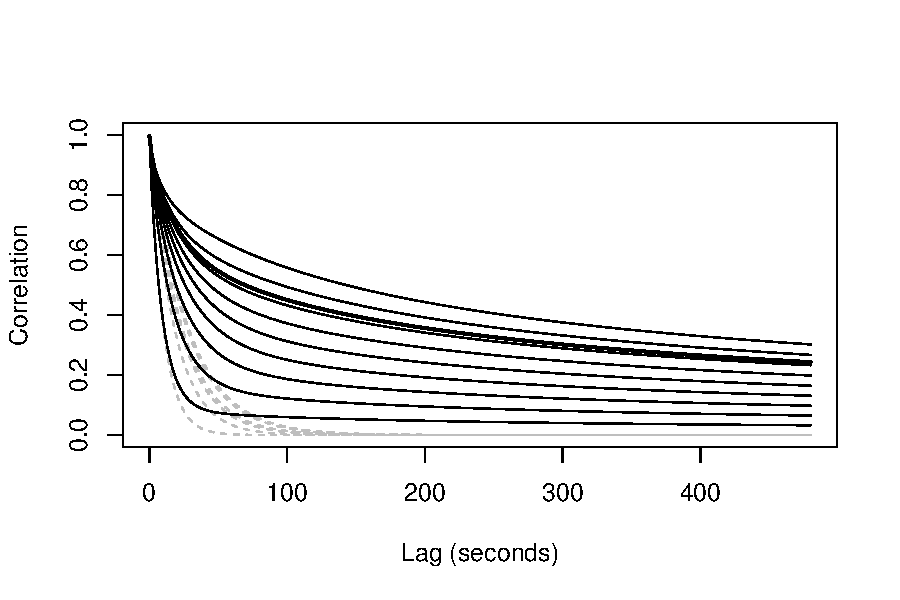
\includegraphics[width=\maxwidth]{figs/fig_correlation_plot-1} 

}

\caption[Correlation between detections by the two observes as a function of lag, for mean proportion of time available (\(\alpha\)) and mean dive cycle duration of \(100\) seconds (dark line)]{Correlation between detections by the two observes as a function of lag, for mean proportion of time available (\(\alpha\)) and mean dive cycle duration of \(100\) seconds (dark line). Gray lines show the correlation for mean proportions of time available of \(47\%, 52\%, 57\%, 62\%, 67\%, 77\%, 82\%, 87\%, 92\%\) and, \(97\%\) seconds. The black line is for \(\alpha=72\%\)}\label{fig:fig_correlation_plot}
\end{figure}


\end{knitrout}



\begin{knitrout}
\definecolor{shadecolor}{rgb}{0.969, 0.969, 0.969}\color{fgcolor}\begin{figure}

{\centering 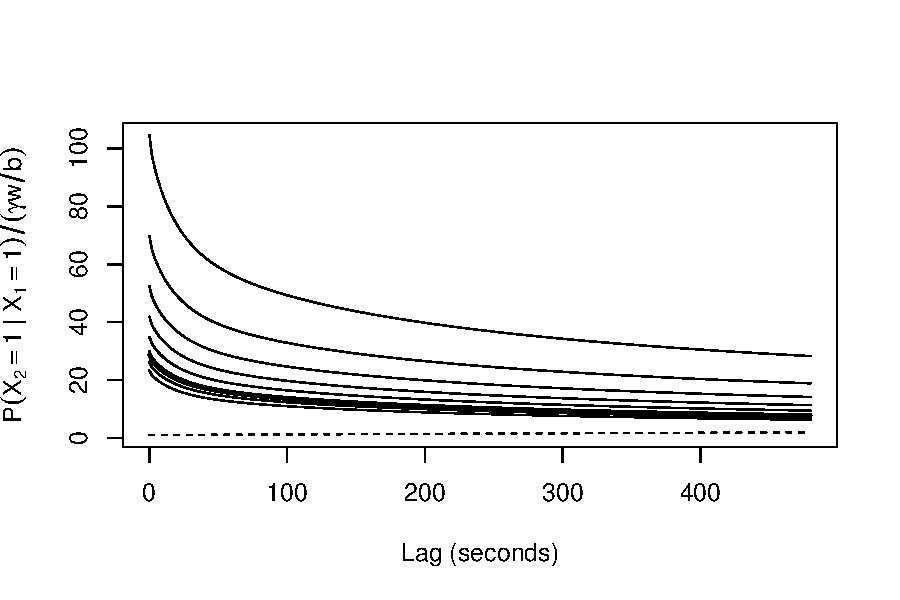
\includegraphics[width=\maxwidth]{figs/fig_p_avail_plot-1} 

}

\caption[The percentage by which the probability of observer 2 detecting an animal given that observer 1 detected it, is greater than the proportion of time animals are available (\(\alpha\))]{The percentage by which the probability of observer 2 detecting an animal given that observer 1 detected it, is greater than the proportion of time animals are available (\(\alpha\)). This is shown for lags from 10 to 100 percent of the dive cycle length. The dark line is for \(\alpha=0.72\).}\label{fig:fig_p_avail_plot}
\end{figure}


\end{knitrout}


\begin{knitrout}
\definecolor{shadecolor}{rgb}{0.969, 0.969, 0.969}\color{fgcolor}\begin{figure}

{\centering 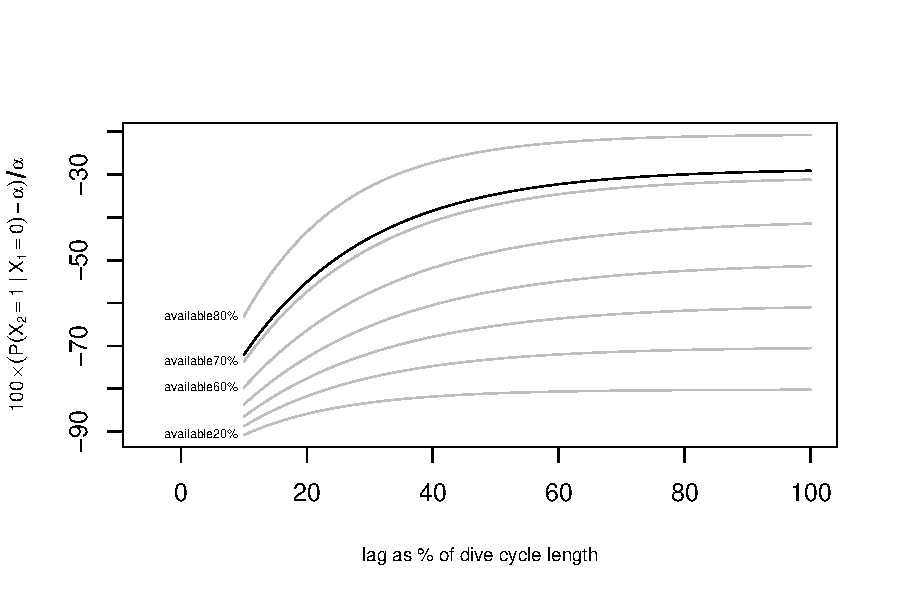
\includegraphics[width=\maxwidth]{figs/fig_p_unavail_plot-1} 

}

\caption[The percentage by which the probability of observer 2 detecting an animal given that observer 1 did not detect it, is greater than the proportion of time animals are available (\(\alpha\))]{The percentage by which the probability of observer 2 detecting an animal given that observer 1 did not detect it, is greater than the proportion of time animals are available (\(\alpha\)). This is shown for lags from 10 to 100 percent of the dive cycle length. The dark line is for \(\alpha=0.72\).}\label{fig:fig_p_unavail_plot}
\end{figure}


\end{knitrout}

On the bases of these figures, we decided to simulate with lag $l$ equal 10\%, 20\%, 50\% and 80\% of dive cycle length and for $\alpha$ equal to 10\%, 20\%, 50\% and 80\%. We do this for three values of $\sigma$, coresponding to mean animal speed of 1.5 m/s \citep[the value estimated by][]{Hiby+Lovell:98}, 0.95 m/s \citep[the value estimated by][]{Westgate+al:95}, and 0.65 m/s \citep[the value estimated by][,which being lower than that which we estimated above, broadens the range of our simulations beyond that were we to use our estimate of $\sigma$]{Stevenson+al:18}. In all cases we simulate with true density $D=1.24$, as estimated in the previous section using our method.

Simulation results are shown in Table~\ref{tab:mlesims}.

% latex table generated in R 3.4.4 by xtable 1.8-2 package
% Tue Nov 13 23:00:57 2018
\begin{table}[ht]
\centering
\caption{Preliminay sims with Nsim=300.} 
\label{tab:mlesims}
\begin{tabular}{rrrrrrr}
  \hline
 & alpha & l & speed & \%Bias & \%CV & \%Cover \\ 
  \hline
1 & 0.10 & 10.00 & 0.65 & 2.20 & 23.22 & 0.96 \\ 
  2 & 0.10 & 10.00 & 0.95 & 3.96 & 24.67 & 0.94 \\ 
  3 & 0.10 & 10.00 & 1.50 & -0.69 & 30.45 & 0.95 \\ 
  4 & 0.10 & 20.00 & 0.65 & 8.13 & 38.77 & 0.95 \\ 
  5 & 0.10 & 20.00 & 0.95 & 8.27 & 33.73 & 0.97 \\ 
  6 & 0.10 & 20.00 & 1.50 & 9.79 & 50.08 & 0.96 \\ 
  7 & 0.10 & 50.00 & 0.65 & 16.65 & 75.51 & 0.83 \\ 
  8 & 0.10 & 50.00 & 0.95 & 18.27 & 64.76 & 0.83 \\ 
  9 & 0.10 & 50.00 & 1.50 & 6.28 & 73.32 & 0.76 \\ 
  10 & 0.10 & 80.00 & 0.65 & 7.76 & 74.05 & 0.77 \\ 
  11 & 0.10 & 80.00 & 0.95 & 11.63 & 73.92 & 0.75 \\ 
  12 & 0.10 & 80.00 & 1.50 & 9.32 & 105.32 & 0.66 \\ 
  13 & 0.20 & 10.00 & 0.65 & 0.73 & 18.42 & 0.97 \\ 
  14 & 0.20 & 10.00 & 0.95 & 1.48 & 20.02 & 0.96 \\ 
  15 & 0.20 & 10.00 & 1.50 & -2.49 & 24.91 & 0.97 \\ 
  16 & 0.20 & 20.00 & 0.65 & 1.27 & 18.92 & 0.96 \\ 
  17 & 0.20 & 20.00 & 0.95 & 2.88 & 19.75 & 0.93 \\ 
  18 & 0.20 & 20.00 & 1.50 & 0.94 & 23.03 & 0.96 \\ 
  19 & 0.20 & 50.00 & 0.65 & 5.26 & 30.59 & 0.96 \\ 
  20 & 0.20 & 50.00 & 0.95 & 9.55 & 38.51 & 0.93 \\ 
  21 & 0.20 & 50.00 & 1.50 & 8.54 & 50.85 & 0.97 \\ 
  22 & 0.20 & 80.00 & 0.65 & 11.25 & 47.62 & 0.91 \\ 
  23 & 0.20 & 80.00 & 0.95 & 12.70 & 52.64 & 0.94 \\ 
  24 & 0.20 & 80.00 & 1.50 & 23.04 & 78.36 & 0.88 \\ 
  25 & 0.50 & 10.00 & 0.65 & 0.66 & 16.75 & 0.97 \\ 
  26 & 0.50 & 10.00 & 0.95 & 1.18 & 19.61 & 0.93 \\ 
  27 & 0.50 & 10.00 & 1.50 & -0.27 & 24.83 & 0.92 \\ 
  28 & 0.50 & 20.00 & 0.65 & 1.38 & 13.75 & 0.96 \\ 
  29 & 0.50 & 20.00 & 0.95 & 1.16 & 14.80 & 0.94 \\ 
  30 & 0.50 & 20.00 & 1.50 & 1.23 & 21.44 & 0.91 \\ 
  31 & 0.50 & 50.00 & 0.65 & 0.56 & 11.96 & 0.96 \\ 
  32 & 0.50 & 50.00 & 0.95 & -0.27 & 14.18 & 0.94 \\ 
  33 & 0.50 & 50.00 & 1.50 & 0.87 & 22.10 & 0.92 \\ 
  34 & 0.50 & 80.00 & 0.65 & -0.66 & 13.88 & 0.95 \\ 
  35 & 0.50 & 80.00 & 0.95 & 1.57 & 15.77 & 0.95 \\ 
  36 & 0.50 & 80.00 & 1.50 & 4.67 & 28.74 & 0.94 \\ 
  37 & 0.80 & 10.00 & 0.65 & 1.69 & 11.95 & 0.92 \\ 
  38 & 0.80 & 10.00 & 0.95 & 2.86 & 12.62 & 0.94 \\ 
  39 & 0.80 & 10.00 & 1.50 & 4.73 & 17.42 & 0.88 \\ 
  40 & 0.80 & 20.00 & 0.65 & 0.57 & 7.78 & 0.95 \\ 
  41 & 0.80 & 20.00 & 0.95 & 0.85 & 8.35 & 0.96 \\ 
  42 & 0.80 & 20.00 & 1.50 & 2.49 & 12.68 & 0.92 \\ 
  43 & 0.80 & 50.00 & 0.65 & 0.47 & 6.04 & 0.98 \\ 
  44 & 0.80 & 50.00 & 0.95 & -0.05 & 7.47 & 0.97 \\ 
  45 & 0.80 & 50.00 & 1.50 & 1.76 & 13.07 & 0.95 \\ 
  46 & 0.80 & 80.00 & 0.65 & -0.35 & 6.61 & 0.99 \\ 
  47 & 0.80 & 80.00 & 0.95 & -0.24 & 7.92 & 0.96 \\ 
  48 & 0.80 & 80.00 & 1.50 & 1.02 & 14.96 & 0.89 \\ 
   \hline
\end{tabular}
\end{table}



Figure~\ref{fig:biascv} shows the relative bias and CV of the maximum likelihood estimator (MLE) of this paper, for each of the simulation scenarios, as a function of propotion of time avaialable ($\alpha$) and lag ($l$). Figue~\ref{fig:mlepalm} compares the relative biases and CVs of the MLE and Palm estimators for each of the simulation scenarios.




\begin{figure}
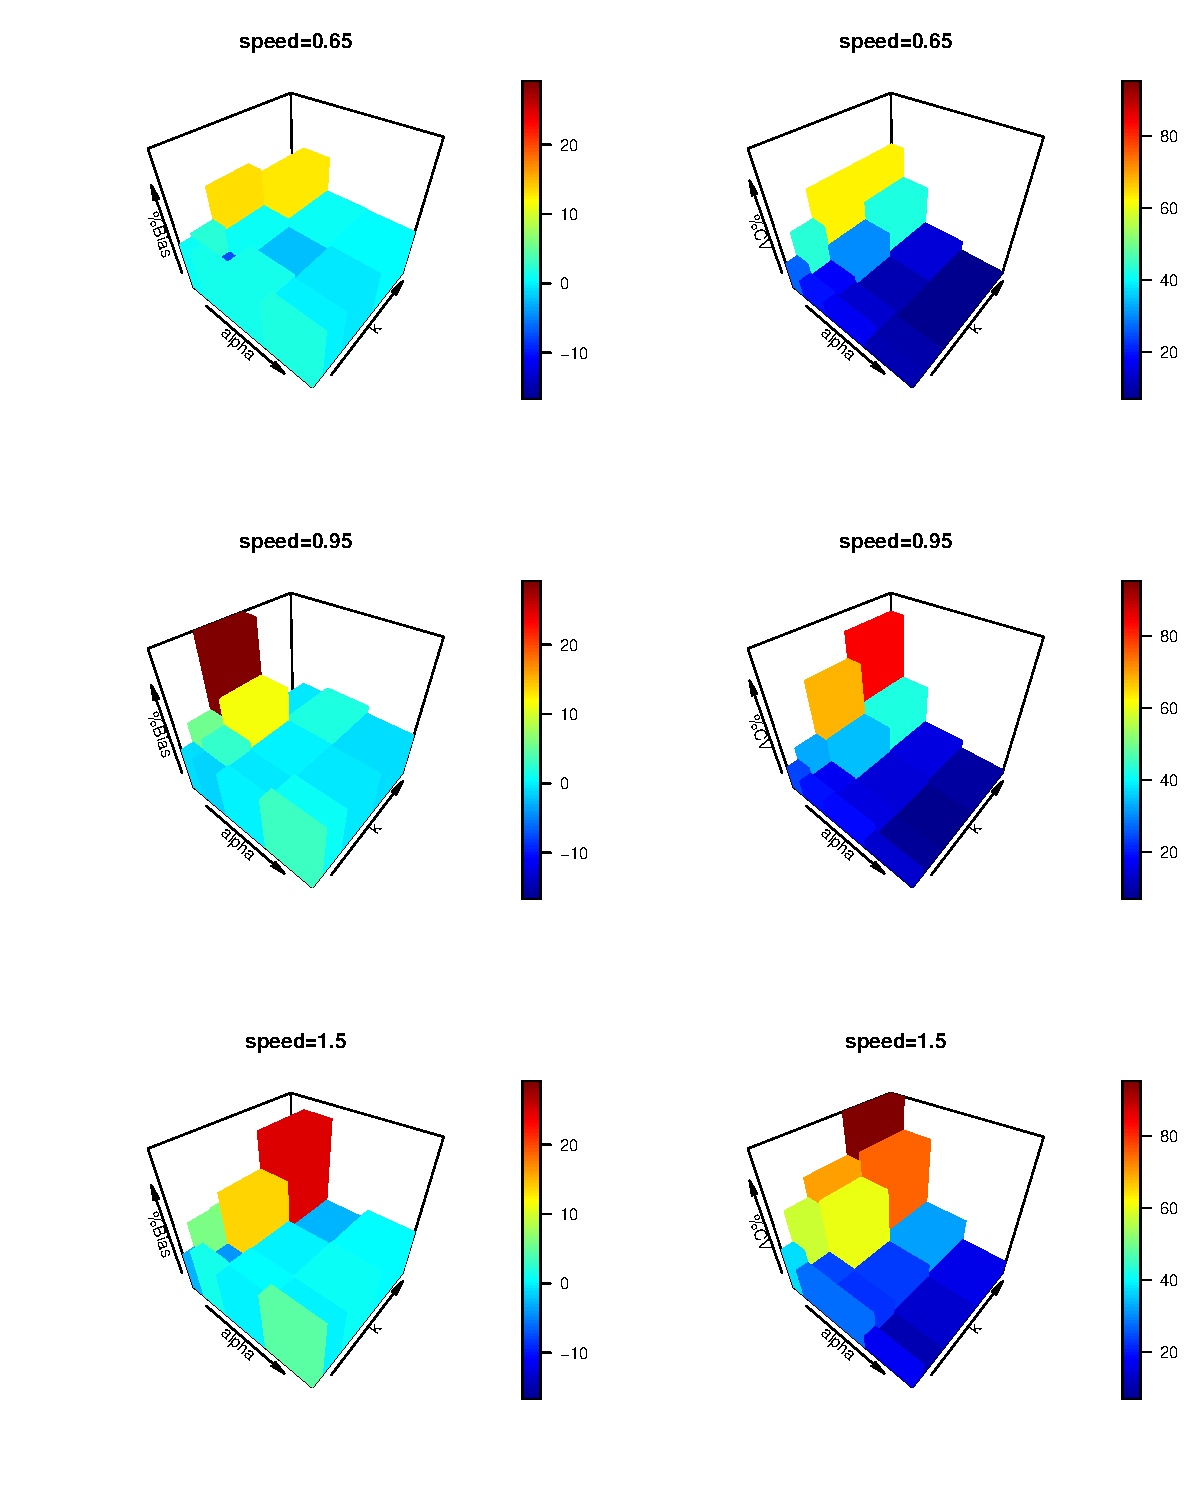
\includegraphics[width = \textwidth]{figs/biascv.pdf}
\caption{The percentage bias (first column) and percentage CV (second column) of $\hat{D}$ as a function of proportion of time available ($\alpha$) and lag ($l$), for each of the three animal speeds considered.}
\label{fig:biascv}
\end{figure}





\begin{figure}
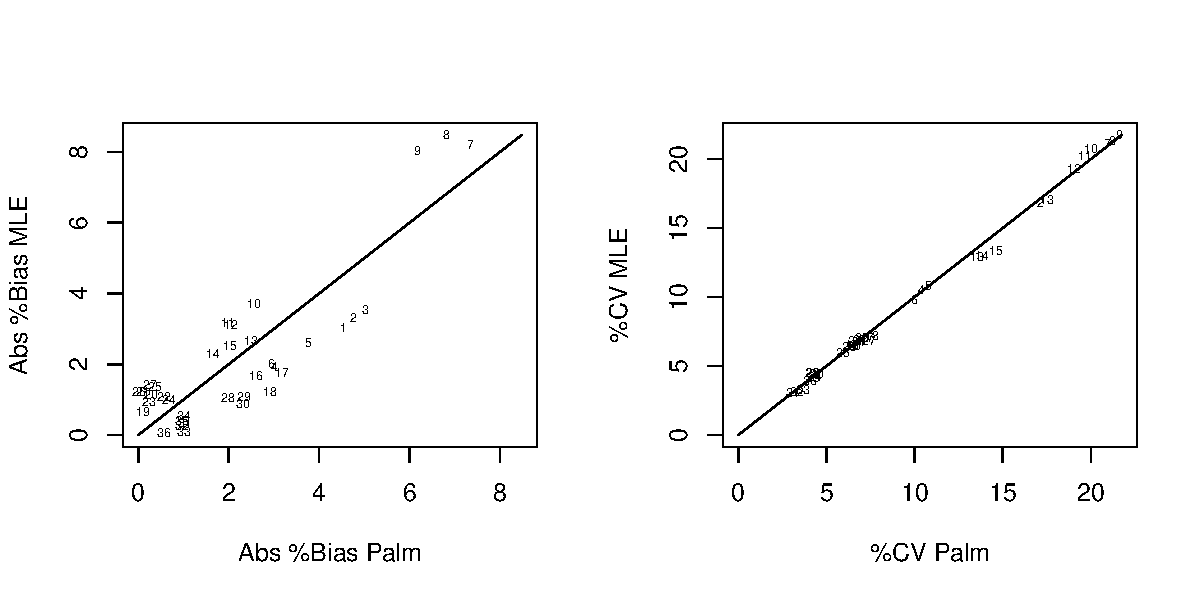
\includegraphics[width = \textwidth]{figs/mlepalm.pdf}
\caption{The percentage bias (left) and percentage CV (right) of the MLE and Palm estimators of $\hat{D}$ over all simulation scenarios. Each point corresponds to one simulation scenario; scenaios with $k=80$ are marked with diamonds, those with $\alpha=0.1$ are marked with crosses. The bias and CV are the same for the two methods along the lines.}
\label{fig:mlepalm}
\end{figure}

Tentative conclusions from this (need larger number simulations to comment further):
\begin{itemize}

\item The MLE is relatively unbiased, except when $\alpha$ is small, and in this case bias gets worse as lag $l$ gets larger. (This seems weird to me - I'd have thought that bias is lowest when $l$ is large! What is going on here?)

\item Similarly, percentage CV is worst when  $\alpha$ is small and lag $l$ is big. (Again weird!)

\item Both MLE and Palm estimators probably almost unbiased.

\item The MLE seems a little more precise than the Palm estimator. Interpretation: Likelihood contains some information that is lost in the Palm likelihood approximation.

\item (Want to include SCR estimator when do fuller set of simulations - to investigate information loss due to lack of recapture identities.)

\end{itemize}


\section{Discussion\label{sec:discussion}}

\begin{itemize}

\item Could estimate $(D,p,\sigma)$ instead of $(D,\mu_1,\sigma)$, if unsure that see all on surface, but then need to assume know $(\mu_1,\tau)$.

\item Varying lag makes one more parameter identifiable (in principle at least). Would be good to expand on this some.

\item Can put covariates into any of the parameters. \textit{Does this make parameters identifiable? Varying lag is effectively this.}

\item With known capture histories this is a kind of SCR transect search with a continuous time movement model and an availability model. Mention difference betwee this and SCR M$_b$ model (and refer to Ben's paper)?

\item If know capture histories, can estimate movement and dive cycle parameters.

\item Slower moving observers: need to take account of first passage time (which ccr method does not).

\item We provide a theoretical structure on which one can build more general modesl for digital survey data, without requiring recapture identification. We anticipate that this could result in very substantial estimation efficiency by allowing the estimation process to be automated. To automate the process we need only an adequate automatic identifier of the species in question in the video stream from each ``observer'' separately. If false negatives affect only the availability process (e.g. remove animals underwater and partially visible), the only cost of using a strict identification criterion in order to avoid false positives, is reduced sample size. If, however, false negatives affect the detection process (e.g. remove some individuals because although they were as available as possible, a wave broke over them as the observer passed) then the assumption of $p=1$ may be violated and bias may ensue. Surveying at different lags will in principle allow estimation of $p$ (in additon to $D$, $\sigma$ and $\mu_1$) so that it will likely be possible to automate inference from digital surveys by using automated object identification criteria that are sufficiently strict so as to reduce the probability of false positives to virtually zero, providing that the survey involves effort and detections at more than one lag.

\end{itemize}



\appendix
%\appendixpage

\section{Derivation of $f_{T}(t)$}
\label{appx:firstpassage}

\todo[inline]{Note to self: need to simplify this - see Rachel's suggestions.}

One can view the poblem of finding the pdf of the time between the first and second observers passing an animal as a the problem of finding the first passage time to a point at distance $vl$ from the origin, of a particle following Brownian motion starting at the origin, with constant drift velocity $v$ and diffusion parameter $\sigma$. We can write the process as $Y_t=\sigma B_t+vt$, where $B$ is a Brownian motion and $Y_t$ is the animal's displacement at time $t$. 

%\todo[inline]{Currently this is based on these two pages: https://math.stackexchange.com/questions/1053294/density-of-first-hitting-time-of-brownian-motion-with-drift and https://math.stackexchange.com/questions/179210/derivation-of-wiener-process-first-passage-times-using-probability-generating-fu}

We use the result \textbf{(citation)} that for $X_t=B_t+ct$, where $B$ is a Brownian motion, a ``boundary'' at $a>0$, and a constant drift rate $c\in\mathbb{R}$, the pdf of $T=\inf\{t: X_t=a\}$ is 
\begin{equation}
f_{T} (t) = \frac{ a \exp \Big\{ \frac{- (a-ct)^2}{2t} \Big\} }{\sqrt{2 \pi t^3}}.
\end{equation}

In our case, we have the ``boundary'' (the second observer) at a distance $vl$ from the starting position of the animal, approaching it at speed $v$, and the animal moving according to brownian motion with parameter $\sigma$, so that $Y_t=\sigma B_t+vt$. If we rescale distance to be in units of $\sigma$, i.e. $X_t=Y_t/\sigma$, we have $X_t=B_t+\frac{v}{\sigma}t$ and $a=vl/\sigma$. Hence the pdf of time to the second observer passing, given that the second observer passes a fixed point at a time $l$ later than the first, is
\be
f_{T} (t)
&=&
\frac{\frac{vl}{\sigma} \exp \Big\{ \frac{- (vl/\sigma-vt/\sigma)^2}{2t} \Big\} }{\sqrt{2 \pi t^3}} 
\;=\;
\frac{vl \exp \Big\{ \frac{- v^2(l-t)^2}{2\sigma^2t} \Big\} }{\sqrt{2 \pi\sigma^2 t^3}}.
\ee


\section{Relationship between $\sigma$ and mean animal speed}
\label{appx:sigmaspd}

We're considering 1-dimensional movement here. Let $X(t)$ be the location of the animal relative to its starting position after time $t$. Then, assuming it starts at $X(0)=0$, $X(t)\sim N(0,\sigma\sqrt{t})$ and $Z(t)=X(t)/[\sigma\sqrt{t}]\sim N(0,1)$. Let $U(t)=\sqrt{Z(t)^2}$. Then\footnote{See \texttt{https://math.stackexchange.com/questions/1059938/whats-the-expectation-of-square-root-of-chi-square-variable}} $U(t)\sim\chi(1)$, with expected value $E[U(t)]=\sqrt{2}\Gamma(1)/\Gamma(1/2)=0.7978846$. Hence an animal moving according to Brownian motion, with parameter $\sigma$, is expected to move a distance $0.7978846\sigma$ per unit time, i.e. have an average speed of $0.7978846\sigma$. Conversely, to model Brownian animal movement in which animals have an average speed of $v$, we need $\sigma=v/0.7978846$. For example, to model animal movement with average speed of 0.95m/s, as in \cite{Stevenson+al:18}, we require $\sigma=0.95/0.7978846$m/s, or $0.95/797.8846\approx 0.00119$km/s.


\bibliographystyle{biom} 
\bibliography{dlb}

%\newpage
%\section*{Online supplementary material}


\end{document}

